% !TEX TS-program = xelatex
% !TEX encoding = UTF-8 Unicode

% This is a simple template for a LaTeX document using the "article" class.
% See "book", "report", "letter" for other types of document.

\documentclass[11pt]{article}

\usepackage[margin=1in]{geometry}
\usepackage{fancyhdr}
\usepackage{framed}
\usepackage{amsmath,amsthm,amssymb}

\usepackage{titlesec}

\usepackage[svgnames]{xcolor}

\usepackage{enumerate}

%\usepackage{mathpazo}
\usepackage{mathtools}
\usepackage{unicode-math}
\usepackage{empheq}
\usepackage[most]{tcolorbox}
 
 \usepackage{hyperref}
 
 \usepackage{caption}

\usepackage{xunicode} %handle unicode
\usepackage{xltxtra} %XeTeX extras
\usepackage{fontspec} %use OTF/TTF fonts


%\newcommand{\lmr}{\fontfamily{lmr}\selectfont} % Latin Modern Roman
%\setmainfont{Myriad Pro} %use this font

\titleformat{\section}
  {\large\bf}{\thesection}{0.25em}{}[\titlerule]
\titlespacing{\section}
  {0pt}{*1.5}{0.25em}

\titleformat{\subsection}
  {\normalfont\bf}{\thesubsection}{0.25em}{}
\titlespacing{\subsection}
  {0pt}{*1}{0.125em}

\renewcommand\thesection{\Alph{section}}

\renewcommand{\labelitemi}{\textemdash}

\DeclareMathOperator{\dif}{d\!}
%\DeclareMathOperator{\Pr}{P}
\DeclareMathOperator{\E}{E}
\DeclareMathOperator{\var}{var}
\DeclareMathOperator{\F}{\mathfrak{F}}
\DeclareMathOperator{\Poisson}{Poisson}
\DeclareMathOperator{\Bernoulli}{Bernoulli}
\DeclareMathOperator{\Binomial}{Binomial}
\DeclareMathOperator{\Order}{O}
\DeclareMathOperator{\Uniform}{Uniform}
\DeclareMathOperator*{\argmax}{argmax}
\DeclareMathOperator{\Tr}{Tr}

\newcommand{\logdet}[1]{\log \left| {#1} \right| }

\newcommand{\xb}{\mathbf{x}}
\newcommand{\ub}{\symbf{\mu}}
\newcommand{\Sb}{\symbf{\Sigma}}

\newcommand*{\tran}{^{\mkern-1.5mu\mathsf{T}}}
\newcommand*{\invtran}{^{\mkern-1.5mu\mathsf{-T}}}

\newenvironment{propertybox}{%
   \def\FrameCommand{\colorbox{LightSteelBlue}}%
   \MakeFramed{\advance\hsize-\width \FrameRestore}}
 {\endMakeFramed}

\lhead{\textbf{ELEC548}}
\chead{Review of Classification}
\cfoot{}
\rhead{}
\rfoot{\thepage}
\pagestyle{fancyplain}

\setlength\parindent{0pt}

\begin{document}
\setmainfont{Myriad Pro} %use this font
\setmathfont{Latin Modern Math}
%\setmathfont{TG Pagella Math}

\begin{center}
\large
\textbf{ELEC 548} Byron's Review of Classification
\end{center}

\section{What is Classification}
Classification is a classic instance of \textbf{supervised learning}. The goal is to define a \textbf{classifier} which properly assigns a new data point -- let's call it $\xb$ -- to the appropriate discrete class $C_k \in \lbrace C_1, \ldots, C_K \rbrace$. While there are solutions to classification problems (i.e., nonparametric) which can be posed when the number of classes, $K$, is not known \textit{a priori} or is otherwise unbounded, below we will assume that it not just countable, but also  finite and typically specified as part of the problem statement. Notice that the discrete number of classes is what makes this a \textit{classification} problem --- the machine learning equivalent for continuous data would generally be termed \textit{regression}. 

The process of solving a a classification problem involves two stages: \textbf{Training}  -- optimizing the classifier using labeled training data, and \textbf{Testing} -- evaluating  the performance of the optimized classifier on labeled testing data. Thus, we always divide our labeled data into two: a test data set to evaluate performance and a separate training  data set to ensure that the classifier we have learned generalizes. (Aside - if we didn't do this, what would be the best performing classifier? A lookup table!)  In cases when there are hyperparameters to be optimized -- for example in the model or statistical distribution of the data -- we can split the labeled data into three groups: a training set, a \textbf{validation} data set to pick the best model, and a test set to evaluate final performance.

Classification is a machine learning problem with a wide variety of formulations and solutions. Below, we review classification using \textbf{Probabilistic Generative Models}. For more information as well as a description of other classification approaches, a good resource is \textit{Pattern Recognition and Machine Learning} by Christopher Bishop.

\begin{figure}[h]
\begin{minipage}{0.45\textwidth}
\textbf{Training Data}

\includegraphics[scale=0.077]{Figure1-TrainingData.jpg}
\end{minipage} \hfill
\begin{minipage}{0.05\textwidth}
\begin{center}
{\Huge $\Rightarrow$}
\end{center}
\end{minipage}
\hfill
\begin{minipage}{0.45\textwidth}
\textbf{Decision Boundaries}

\includegraphics[scale=0.077]{Figure2-DecisionBoundaries.jpg}
\end{minipage}
\caption{The classification problem involves taking this training data and finding decision boundaries for new data points.}
\end{figure}




\section{Classification Using Probabilistic Generative Models}
In a classifier built using a probabilisitic generative model, there are two densities for each class $k \in \lbrace 1, \ldots, K\rbrace$:
\begin{itemize}
\item the class-conditional density, $\Pr \left(\xb \mid C_k\right)$ and
\item the class priors $\Pr \left(C_k\right)$
\end{itemize}

To \textbf{train} the classifier, we can use \textit{maximum likelihood parameter estimation}. To use the classifier (i.e., on \textbf{test} data), we chose the class which maximizes the \textit{a posteriori} probability. In other words, we
\begin{itemize}
\item use Bayes' rule to compute $\Pr \left(C_k \mid \xb\right)$
\begin{equation}
    \begin{split}
        \Pr \left(C_k \mid \xb\right) &= \frac{\Pr\left(\xb \mid C_k\right) \Pr\left(C_k\right)}{\Pr\left(\xb\right)} \\
                    &= \frac{\Pr\left(\xb \mid C_k\right) \Pr\left(C_k\right)}{\sum_{i=1}^{K} \Pr\left(\xb \mid C_i\right) \Pr\left(C_i\right)} 
    \end{split}
\end{equation}

\item assign $\xb$ to class $C_m$ where
\begin{equation}
	m = \argmax_k \Pr \left(C_k \mid \xb\right)
 \end{equation}
\end{itemize}

\subsection{Philosophy of Probabilistic Generative Models}
$\Pr(\xb \mid C_k)$ and $\Pr(C_k)$ define a ``probabilistic generative model'' (or just ``generative model''). Unlike other classification schemes, this means
that we can generate synthetic data using our model. 

For example, imagine there are two classes and $\xb \in \mathbb{R}^2$. 
\begin{flalign*}
	\Pr(C_1) = 0.7 \\
	\Pr(C_2) = 0.3 \\
	\Pr(\xb \mid C_1) = \mathcal{N} \Bigl(
		\begin{bmatrix} 2 \\ 1 \end{bmatrix}, 
		\begin{bmatrix} 1 & 0 \\ 0 & 1 \end{bmatrix} \Bigr) \\
	\Pr(\xb \mid C_2) = \mathcal{N} \Bigl(
		\begin{bmatrix} 1 \\ 2 \end{bmatrix}, 
		\begin{bmatrix} 1 & 0 \\ 0 & 1 \end{bmatrix} \Bigr) \\		
\end{flalign*}
To generate synthetic data from this model begin by sampling from your handy $\text{Uniform}[0,1)$ random number generator.
\begin{itemize}
	\item If the uniform r. v. sample is $< 0.7$, draw a data sample from the Gaussian $\Pr(\xb \mid  C_1)$.
	\item If the uniform r. v. sample is $\geq 0.7$, draw a data sample from the Gaussian $\Pr(\xb \mid  C_2)$.
\end{itemize}
(Note that this is the same as flipping a biased coin with probability of heads being 0.7.)

\begin{center}
%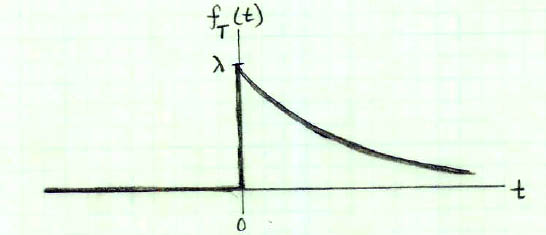
\includegraphics[scale=0.5]{Figure1.jpg}
\end{center}

\textbf{Philosophical point:} If we generate synthetic data from our model and it resembles the real data we are trying to classify,
then we can have some confidence that our model of the data is good. This will mean that our classifier will be functional and we
can make inferences, decisions, etc.

\subsection{Maximum Likelihood Parameter Estimation}
Once we write down the \textit{training data likelihood}, maximum likelihood parameter estimation is not complicated. What is the data likelihood? Let us assume we are given training data: $\lbrace \xb_n, t_n \rbrace, \quad n = 1, \ldots, N$, where for each of the $N$ training data, $t_n$ is the label for data point $x_n$. Then, the \textit{data likelihood} is just:
\begin{center}
\begin{minipage}{0.75\linewidth}
\begin{propertybox}
    \textbf{Data Likelihood}
    \begin{equation}
    	\begin{split}
	    	\mathcal{L} &\equiv \Pr \left( \lbrace\xb_n, t_n\rbrace \mid \symbf{\theta} \right)  \\
		 	&= \prod_{i=1}^{N} \sum_{k=1}^K \Pr \left( \xb_n \mid C_k , \symbf{\theta} \right) \Pr \left( t_n = k \mid C_k, \symbf{\theta}\right) \delta(t_n = k)
	\end{split}
    \end{equation}
    where $\symbf{\theta}$ are the parameters of the densities and $\delta(t_n = k) = 1$ if $t_n = k$ and $0$ otherwise.
\end{propertybox}
\end{minipage}
\end{center}

 
With a probabilistic generative model approach, in general, we will choose the parameters $\symbf{\theta}$ that maximize the data likelihood (maximum likelihood parameter estimation).

\begin{framed}
\subsubsection*{\underline{Example:} Two classes with Gaussian class-conditional density and shared covariance}

\textbf{Training data:} $\lbrace \xb_n, t_n \rbrace, \, n = 1, \ldots, N$ where
\begin{flalign*}
\quad t_n &= 1 \, \text{denotes membership in} \, C_1 \text{and} &\\
\quad t_n &= 0 \, \text{denotes membership in} \, C_2
\end{flalign*}
\begin{flalign*}
\text{Let} \, & \Pr(t_n = 1) = \Pr(C_1) = \pi &\\
 & \Pr(t_n = 0) = \Pr(C_2) = (1- \pi)
 \end{flalign*}

For a data point $\xb_n \in \mathbb{R}^D$, 
\begin{align*}
\Pr(\xb_n, C_1) &= \Pr(\xb_n \mid C_1) \Pr(C_1) = \mathcal{N}(\xb_n \mid \ub_1, \Sb) \cdot \pi \\
\Pr(\xb_n, C_2) &= \Pr(\xb_n \mid C_2) \Pr(C_2) = \mathcal{N}(\xb_n \mid \ub_2, \Sb) \cdot (1- \pi)  
 \end{align*}

The data likelihood for $N$ data points is then 
\begin{equation}
	\begin{split}
		\mathcal{L} &\equiv \Pr \left( \lbrace\xb_n, t_n\rbrace \mid \symbf{\theta} \right)  \\
		 	&= \prod_{i=1}^{N} \Big(\mathcal{N}(\xb_n \mid \ub_1, \Sb) \cdot \pi\Big)^{t_n} 
			\Big(\mathcal{N}(\xb_n \mid \ub_2, \Sb) \cdot \pi\Big)^{1-t_n}
	\end{split}
\end{equation}
\begin{equation}
	\begin{split}
		\log \mathcal{L} &= \sum_{i=1}^{N} \Big[   t_n \log \left(\mathcal{N}(\xb_n \mid \ub_1, \Sb)\right)  + t_n \log(\pi)  \, +  \\
			& \quad \quad  \quad \quad  (1- t_n) \log \left(\mathcal{N}(\xb_n \mid \ub_2, \Sb)\right)  + (1 - t_n) \log(1 - \pi)  \Big]
	\end{split}
\end{equation}

where
\begin{equation}
	\begin{split}
	& \log \left(\mathcal{N}(\xb_n \mid \ub _k, \Sb)\right) =  \\ 
		&\quad \quad -\frac{1}{2} (\xb_n  - \ub_k)\tran \Sb^{-1} (\xb_n  - \ub_k)
		- \frac{1}{2} \logdet{\Sb}- \frac{D}{2} \log(2 \pi)
	\end{split}
\end{equation}

\subsubsection*{(i) Find $\pi$}
Our goal is to find the value of \pi which maximizes $\mathcal{L}$. Because of the way we've formulated the problem this is
simple calculus - take the gradient and set equal to zero.

\begin{gather*}
	\frac{\partial \log \mathcal{L}}{\partial \pi} = \sum_{n=1}^N \Big[ t_n \cdot \frac{1}{\pi} - (1 - t_n) \cdot \frac{1}{1 - \pi} \Big] = 0 \\
	\frac{1}{\pi} \sum_{n=1}^{N} t_n - \frac{1}{1-\pi} \sum_{n=1}^N (1 - t_n) = 0 \\
	\intertext{Let $N_1 = $ the number of points from $C_1$ in the training data set: $N_1 = \sum_{n=1}^N t_n$, similarly $N_2 = \sum_{n=1}^N (1 -  t_n) = N - N_1$ .}
	\frac{1}{\pi} N_1 - \frac{1}{1-\pi} (N - N_1) = 0 \\
	(1 - \pi) N_1 = \pi (N - N_1)  \\
\end{gather*}
\begin{equation}
	\tcboxmath{\pi = \frac{N_1}{N}}
\end{equation}

What this means is that the maximum likelihood estimate of the class prior probabilities are just the fraction of the training data assigned to each class. 


\subsubsection*{(i) Find $\ub_1$}
 Because of the way we've formulated the problem this is still simple calculus - take the gradient and set equal to zero. 
 If you're not familiar with quadratic forms, take a look at the table of useful matrix calculus identities at the end.

\begin{align*}
	\frac{\partial \log \mathcal{L}}{\partial \ub} &= \frac{\partial}{\partial \ub}  \sum_{i=1}^{N} \Big[   t_n \log \left(\mathcal{N}(\xb_n \mid \ub_1, \Sb)\right)  + t_n \log(\pi)  \, +  \\
			 & \quad \quad  \quad \quad  (1- t_n) \log \left(\mathcal{N}(\xb_n \mid \ub_2, \Sb)\right)  + (1 - t_n) \log(1 - \pi)  \Big] \\
	\intertext{Keeping only the terms that depend on $\ub_1$:} \\
	&= \frac{\partial}{\partial \ub}  \sum_{i=1}^{N} \Big[   t_n \log \left(\mathcal{N}(\xb_n \mid \ub_1, \Sb)\right)   \Big] \\
	&= \frac{\partial}{\partial \ub}  \sum_{i=1}^{N} \Big[   - t_n  \frac{1}{2} (\xb_n  - \ub_1)\tran \Sb^{-1} (\xb_n  - \ub_1)  \Big] \\
	& = - \sum_{n=1}^{N} \Big(t_n \frac{1}{2}  2  \Sb^{-1} (\xb_n - \ub_1) \Big) = 0 \\
	&\implies \Sb^{-1} \sum_{n=1}^{N} \Big(t_n  \xb_n  \Big) = \Sb^{-1} \Big(  \ub_1  \sum_{n=1}^{N} t_n \Big)
\end{align*}
\begin{equation}
	\tcboxmath{\ub_1 = \frac{1}{N_1} \sum_{n=1}^N t_n \xb_n} 
\end{equation}
Similarly, for $\ub_2$:
\begin{equation}
	\tcboxmath{\ub_2 = \frac{1}{N - N_1} \sum_{n=1}^N (1 - t_n) \xb_n}
\end{equation}

So what we've shown is that the maximum likelihood estimate of the class means are the sample means of the training data assigned to each class.

\subsubsection*{(i) Find $\Sb$}
Keeping only the terms that depend on $\Sb$:
\begin{align*}
	\log \mathcal{L} &=  \sum_{i=1}^{N} \Big[   t_n \log \left(\mathcal{N}(\xb_n \mid \ub_1, \Sb)\right)   +  (1 - t_n) \log \left(\mathcal{N}(\xb_n \mid \ub_2, \Sb)\right) \Big] \\
	& =  \sum_{i=1}^{N} \Big[   - t_n  \Big(\frac{1}{2} (\xb_n  - \ub_1)\tran \Sb^{-1} (\xb_n  - \ub_1)  - \frac{1}{2} \logdet{\Sb} \Big)   \\
	 & \quad \quad \quad  - (1 - t_n)  \Big( \frac{1}{2} (\xb_n  - \ub_2)\tran \Sb^{-1} (\xb_n  - \ub_2) - \frac{1}{2} \logdet{\Sb} \Big)  \Big]  \\
	 & =  \sum_{i=1}^{N} \Big[   -  \frac{t_n }{2} \Big( \Tr \Big(\Sb^{-1} (\xb_n  - \ub_1)  (\xb_n  - \ub_1)\tran \Big) - \logdet{\Sb} \Big)   \\
	 & \quad \quad \quad   - \frac{1 - t_n}{2}  \Big(   \Tr \Big(\Sb^{-1} (\xb_n  - \ub_2)  (\xb_n  - \ub_2)\tran \Big) - \logdet{\Sb} \Big)  \Big]  \\
	\frac{\partial \mathcal{L}}{\partial \Sb} &= 	  \sum_{i=1}^{N} \Big[   -  \frac{t_n }{2} \Big( - \Sb^{-1} (\xb_n  - \ub_1)  (\xb_n  - \ub_1)\tran \Sb^{-1}  - \Sb^{-1} \Big)   \\
	 & \quad \quad \quad   - \frac{1 - t_n}{2}  \Big(  - \Sb^{-1} (\xb_n  - \ub_2)  (\xb_n  - \ub_2)\tran \Sb^{-1} - \Sb^{-1} \Big)  \Big]  \\
	 & = 0 \\
\intertext{If we left and right multiply by $\Sb$,} \\
	0 &= \sum_{i=1}^{N} \Big[   \frac{t_n }{2} \Big(  (\xb_n  - \ub_1)  (\xb_n  - \ub_1)\tran  - \Sb \Big)   +  \frac{1 - t_n}{2}  \Big(  (\xb_n  - \ub_2)  (\xb_n  - \ub_2)\tran  - \Sb \Big)  \Big] 
 \end{align*}
Note that the labels, $\lbrace t_n\rbrace$ select which of the two terms are actually calculated for each data point. Also getting rid of the $\frac{1}{2}$ terms, we can write this as
\begin{align*}
	0 &= \sum_{n \in C_1} \Big(  (\xb_n  - \ub_1)  (\xb_n  - \ub_1)\tran  - \Sb \Big)   +  \sum_{n \in C_2}  \Big(  (\xb_n  - \ub_2)  (\xb_n  - \ub_2)\tran  - \Sb \Big)  \\
	0 &= \sum_{n \in C_1} (\xb_n  - \ub_1)  (\xb_n  - \ub_1)\tran  - N_1 \Sb  + \sum_{n \in C_2}  (\xb_n  - \ub_2)  (\xb_n  - \ub_2)\tran  - N_2 \Sb   \\
 \end{align*}
 Thus,
 \begin{equation}
	\tcboxmath{
	\begin{split}
		\Sb &= \frac{N_1}{N} \mathbf{S}_1 + \frac{N_2}{N} \mathbf{S}_2 , \text{where} \\
		& \quad \mathbf{S}_1 = \frac{1}{N_1}  \sum_{n \in C_1} (\xb_n  - \ub_1)  (\xb_n  - \ub_1)\tran \\
		& \quad \mathbf{S}_2 = \frac{1}{N_1}  \sum_{n \in C_2} (\xb_n  - \ub_2)  (\xb_n  - \ub_2)\tran
	\end{split}}
\end{equation}

So what we've shown is that the maximum likelihood estimate of the shared covariance matrix is a weighted sum of the  sample covariances of each of the classes 
($\mathbf{S}_1$ and $\mathbf{S}_2$) where the weighting  by the fraction of points in each class.  These three results make sense intuitively - absent any other 
information, the sample estimates of the training data will be the best estimates of the parameters. 
\end{framed}

\subsection{Test Phase: Assigning a new data point to a class}
Once we have trained our model, we will want to assign data to the best class. As discussed in lecture, aspects of the problem might imply cost/loss functions that 
would result in biased assignments. Absent these considerations, the best assignment is the \textit{maximum a posteriori} class.

\begin{center}
\begin{minipage}{0.75\linewidth}
\begin{propertybox}
    \textbf{MAP Assignment}
    \begin{align}
		\hat{k} &= \argmax_m \Pr (C_m \mid \xb ) \nonumber \\
		&= \argmax_m  \frac{\Pr (\xb \mid C_m) \Pr (C_m)}{\Pr (\xb)} \nonumber \\
		&= \argmax_m \Pr (\xb \mid C_m) \Pr (C_m) \nonumber \\
		&= \argmax_m \log \Pr (\xb \mid C_m) + \log \Pr (C_m) 
    \end{align}
\end{propertybox}
\end{minipage}
\end{center}
where we've simplified by dropping the $\Pr(\xb)$ term, which is common to all classes. 

\begin{framed}
\subsubsection*{\underline{Example cont'd:} Assignment for 2 Gaussians with shared covariance}
For the example of two classes with class-conditional Gaussian densities with a shared covariance matrix, we can further simplify by dropping all the terms which are common
to both classes
\begin{align}
	\hat{k} &= \argmax_m \; \Pr (C_m \mid \xb ) \nonumber \\
	&= \argmax_m \; \log \Pr (\xb \mid C_m) + \log \Pr (C_m) \nonumber  \\
	&= \argmax_m \;  \underbrace{\bigl( \ub_m\tran \Sb^{-1} \xb - \frac{1}{2}\ub_m\tran \Sb^{-1} \ub_m + \log \Pr (C_m) \bigr)}_{\mathrlap{\text{call this $a_m(\xb)$}}}
	\label{eqn:decisionboundary}
\end{align}

This function creates a decision boundary in $\xb$ space. What does it look like?
\end{framed}


\section{Hyperplanes}
\begin{minipage}{0.575 \textwidth}
A hyperplane is the $D$-dimensional generalization of a line in 2-dimensional space and a plane in 3-dimensional space.

A hyperplane is defined as the set of all $\xb$ such that
\begin{equation}
	y(\xb) = \mathbf{w}\tran \xb + w_0 = 0.
	\label{eqn:hyperplane}
\end{equation}
Here, $\mathbf{w}$ determines the \textbf{direction} of the hyperplane and $w_0$ determines the offset from the origin. 
An example in 2-dimensions is to the right in Figure \ref{fig:hyperplane}.
\end{minipage}\hfill
\begin{minipage}{0.4 \textwidth}
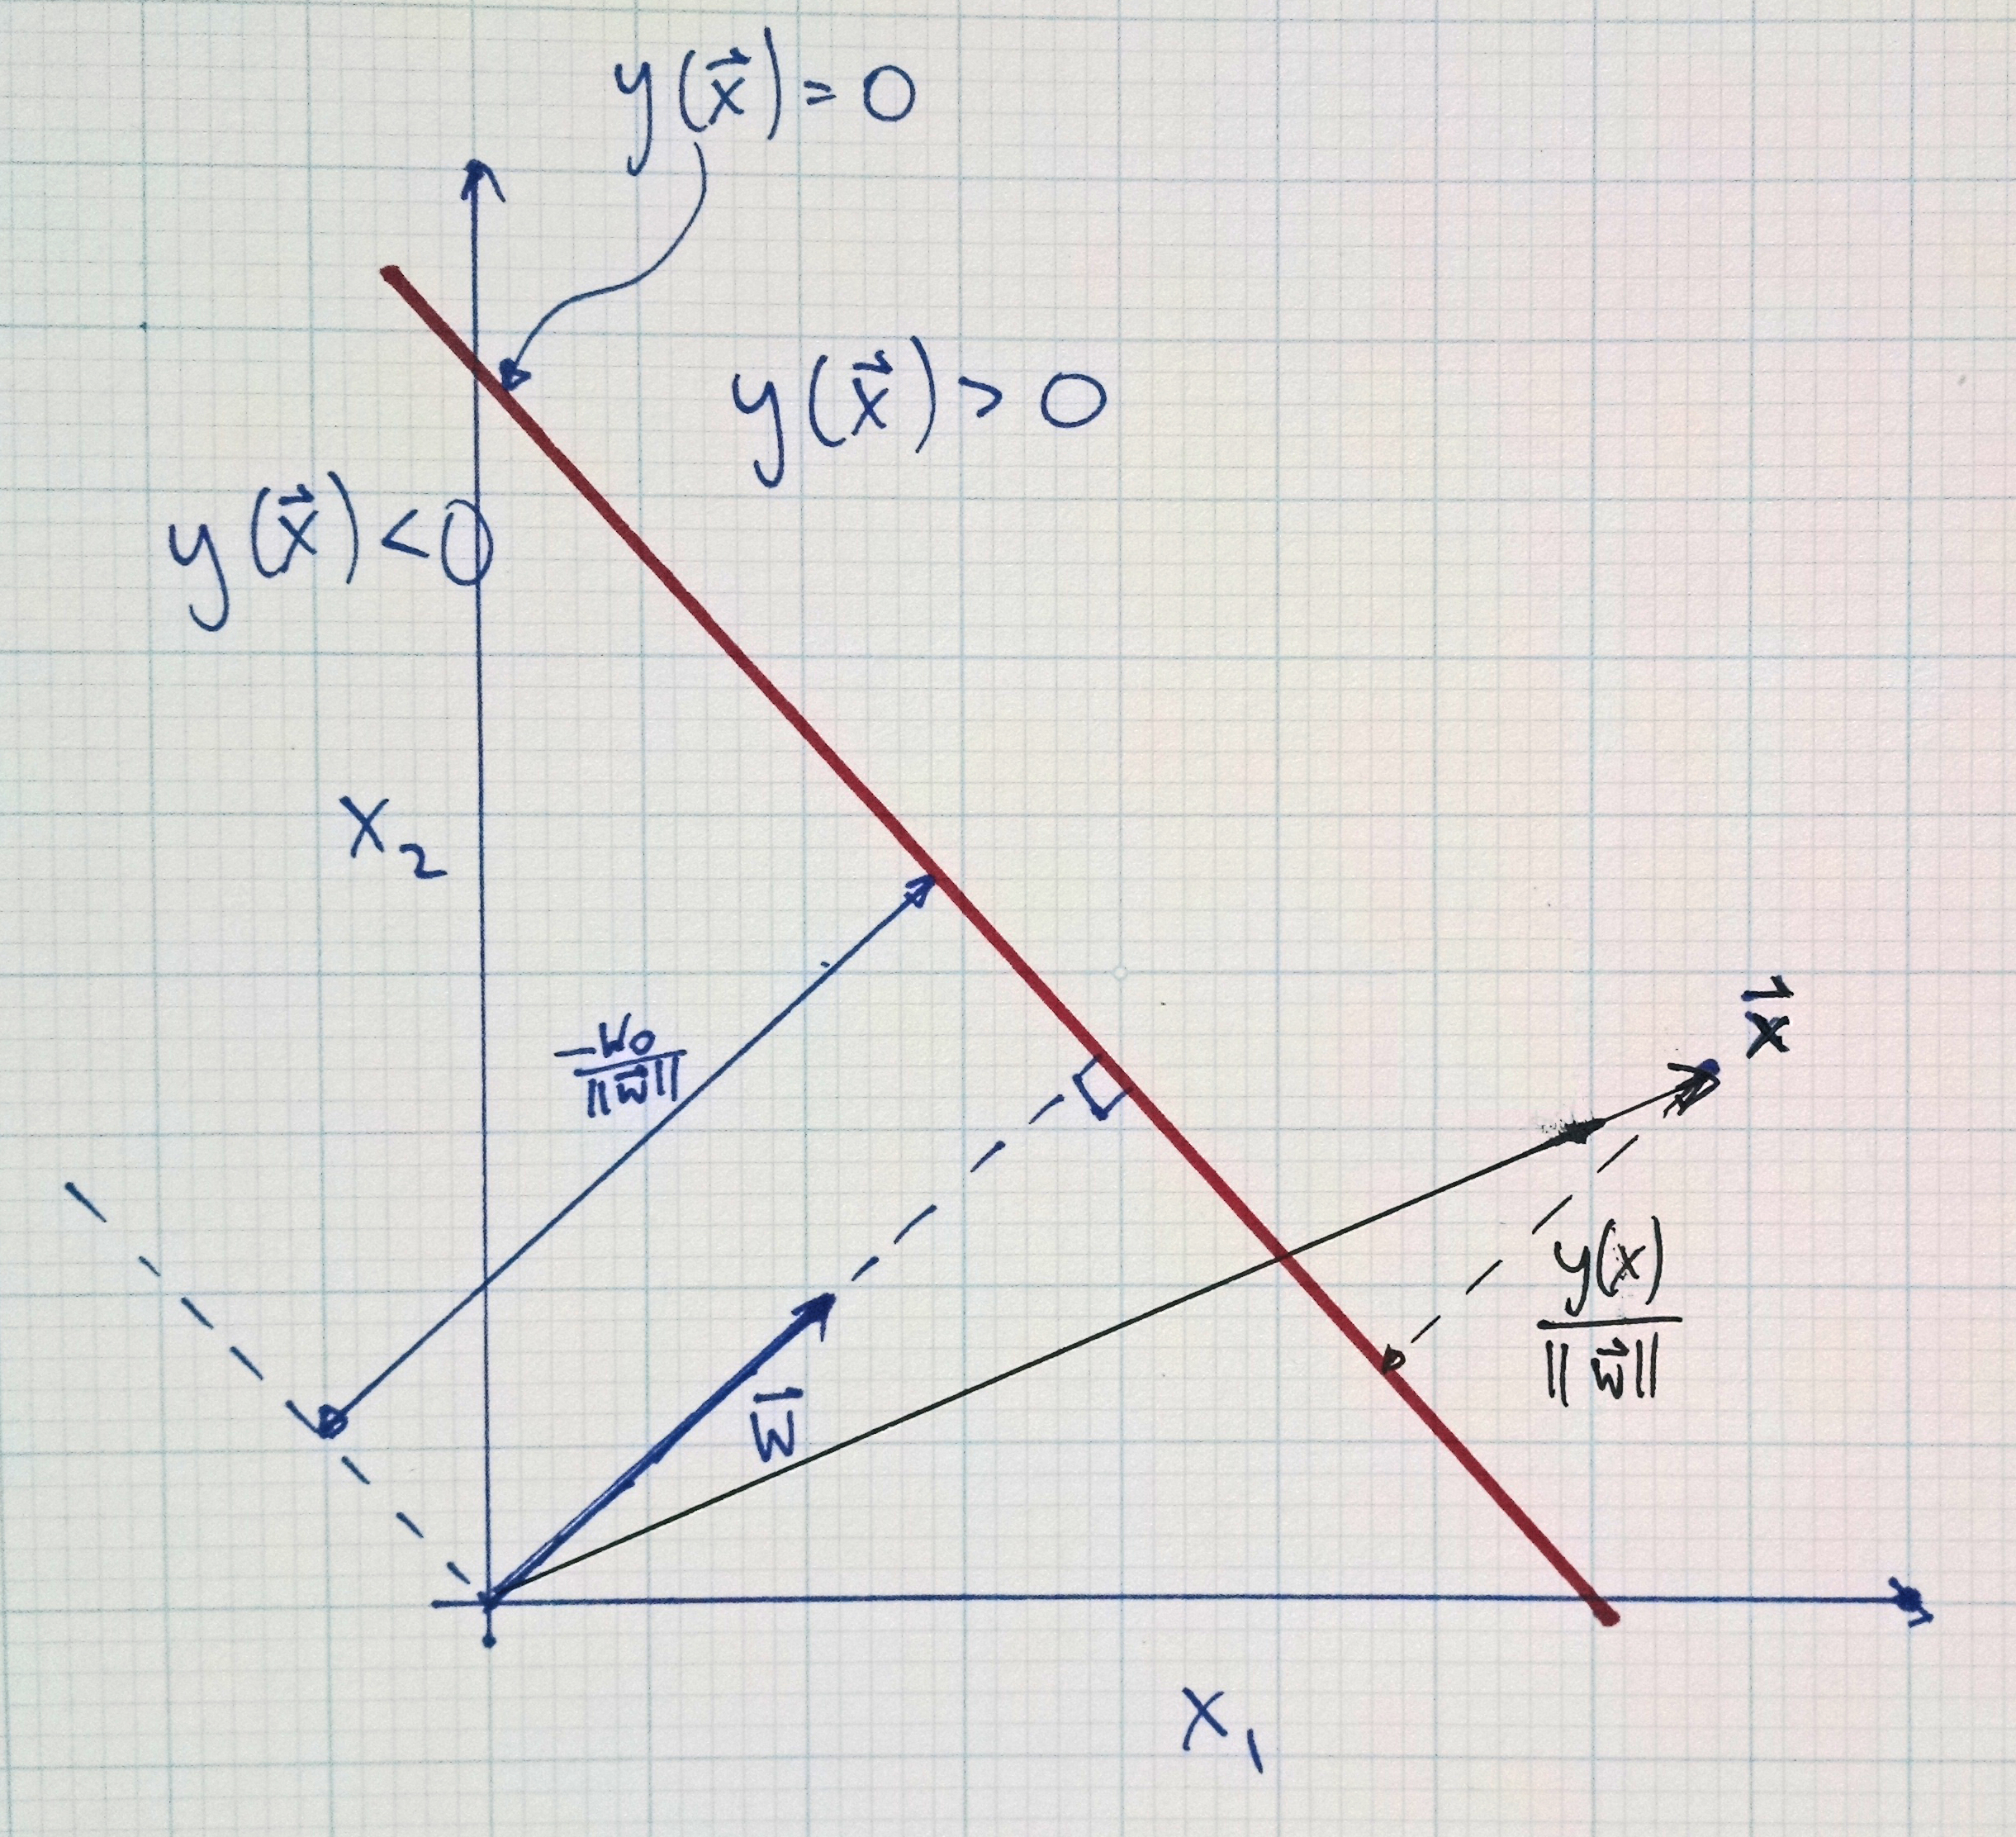
\includegraphics[width=\textwidth]{Figure4-Hyperplane.jpg}
\captionof{figure}{Hyperplane in 2D}
\label{fig:hyperplane}
\end{minipage}

\textbf{Hyperplane Facts:}
\begin{enumerate}
\item \underline{$\mathbf{w}$ is \textit{orthogonal} to the hyperplane it defines.}
\begin{gather*}
	\intertext{Consider two points, $\xb_A$ and $\xb_B$ which lie on a hyperplane.}  \\
	y(\xb_A) = y(\xb_B)  = 0 \\
	\mathbf{w}\tran \xb_A + w_0 = \mathbf{w}\tran \xb_B + w_0 \\
	\mathbf{w}\tran \underbrace{(\xb_A - \xb_B)}_{\mathrlap{\text{a vector lying in the hyperplane}}} = 0 \\
	\implies  \mathbf{w} \; \text{is orthogonal to any vector lying in the hyperplane.}
\end{gather*}

\item \underline{The normal distance from the origin to the hyperplane is} $-\dfrac{w_0}{\lVert \mathbf{w} \rVert}$.
\begin{gather*}
	\intertext{Let $\xb$ be a point on the hyperplane}  \\
	\implies \mathbf{w}\tran \xb + w_0 = 0 \\
	\intertext{The normal distance to the plane is the projection of this (arbitrary vector) $\xb$ onto $\mathbf{w}$} \\
	\bigl( \frac{\mathbf{w}}{\lVert\mathbf{w}\rVert} \bigr)\tran \xb  = - \frac{w_0}{\lVert\mathbf{w}\rVert} _{//}
\end{gather*}

\item \underline{The normal distance from any point $\xb$ to the hyperplane is} $\dfrac{y(\xb)}{\lVert \mathbf{w} \rVert}$.
\begin{gather*}
	\intertext{Project $\xb$ onto $\mathbf{w}$, then subtract $\frac{\mathbf{w}}{\lVert\mathbf{w}\rVert}$.}  \\
	\bigl( \frac{\mathbf{w}}{\lVert\mathbf{w}\rVert} \bigr)\tran \xb + \frac{\mathbf{w}}{\lVert\mathbf{w}\rVert} = \frac{y(\xb)}{\lVert\mathbf{w}\rVert}_{//}
\end{gather*}
\end{enumerate}

\section{Linear Decision Boundaries}
In our example problem, in equation \eqref{eqn:decisionboundary}, a point $\xb$ is assigned to class $C_k$ if $a_k(\xb) > a_j(\xb)$ for all $j \neq k$. Thus, the \textbf{decision boundary} between class $C_k$ and class $C_j$ is given by $a_k(\xb) = a_j(\xb)$.

\begin{align*}
	\intertext{As above, we can define $a_k(\xb) = \mathbf{w}_k\tran \xb + w_{k0}$, where}
	\mathbf{w}_k &= \Sb^{-1} \ub_k \\
	w_{k0} &= - \frac{1}{2} \ub_k \tran \Sb^{-1} \ub_k + \log \Pr(C_k)
\end{align*}
The decision boundary is thus
\begin{equation}
	(\mathbf{w}_k - \mathbf{w}_j)\tran \xb + (w_{k0} - w_{j0})  = 0.
\end{equation}
Note that this is the same form as \eqref{eqn:hyperplane}, and thus the decision boundary \textit{in the case of Gaussian classes 
with a shared covariance matrix} is a $(D-1)$-dimensional hyperplane in $\mathbb{R}^D$.

\section*{Appendix: Useful Matrix Properties and Calculus Identities}
$\quad$
\begin{center}
\begin{minipage}{0.75\linewidth}
\textit{Derivative of a quadratic form for vector $\xb$}
\begin{equation}
	\begin{split}
	\frac{\partial}{\partial \xb} \xb\tran \mathbf{A} \xb &= (\mathbf{A} + \mathbf{A}\tran) \, \xb \\
	&= 2 \mathbf{A} \xb \; \text{when $\mathbf{A}$ is symmetric}
	\end{split}
\end{equation}

\textit{Derivative of a matrix product for matrix $\mathbf{X}$}
\begin{equation}
	\frac{\partial}{\partial \mathbf{X}} \Tr(\mathbf{X}^{-1} \mathbf{A}) = -\mathbf{X}\invtran \mathbf{A}\tran \mathbf{X}\invtran
\end{equation}

\textit{Derivative of the determinant of $\mathbf{X}$}
\begin{equation}
	\frac{\partial}{\partial \mathbf{X}} \logdet{\mathbf{X}} = \mathbf{X}\invtran
\end{equation}

\textit{Invariance of matrix trace to rotation}	
\begin{equation}
	\Tr(\mathbf{A} \mathbf{B} \mathbf{C} \mathbf{D} \ldots) = \Tr(\mathbf{B} \mathbf{C} \mathbf{D} \ldots \mathbf{A}) = 
	\Tr(\mathbf{C} \mathbf{D} \ldots \mathbf{A}  \mathbf{B}) = \ldots
\end{equation}

You will find more on the wikipedia "Matrix calculus" page or by searching for the \
\href{http://www.ee.ic.ac.uk/hp/staff/dmb/matrix/intro.html}{"matrix reference manual"}.
\end{minipage}
\end{center}


\end{document}


